\documentclass{article}
\usepackage{amsmath, amsfonts, graphicx}
\begin{document}
\section{Problem Statement}
We consider a special type of piecewise affine system, that the boundaries of the hybrid modes intersect at the origin. Mathematically, the system has this form
\begin{align}
	\dot{x} = f(x) = A_ix \text{ if } P_ix\le 0
\end{align}
Notice that the righ-hand side of $P_ix\le0$ is zero vector, which guarantees that all mode boundaries pass through the origin. This also implies that $f(kx) = kf(x)$ if $k>0$.

We want to find a Lyapunov function satisfying
\begin{align}
	V(x) > 0 \forall x\neq 0\\
	\dot{V}(x) < 0 \forall x\neq 0\\
	V(x) = 0
\end{align}

\textbf{Goal}: We want to prove that if there exists a piecewise affine Lyapunov function in the form 
\begin{align}
	V(x) = g_i^Tx + h_i \text{ if } C_ix\le d_i \label{eq:piecewise_affine_lyapunov}
\end{align}
Namely in the $i'th$ piece $\mathcal{P}_i=\{x | C_ix \le d_i\}$, the Lyapunov function is an affine function of state $x$. Then there has to exist a piecewise linear Lyapunov function in the form
\begin{align}
	\bar{V}(x) = \bar{g}_i^Tx \text{ if } \bar{C}_i x \le 0
\end{align}
Namely the piecewise linear Lyapunov function $\bar{V}$ is linear inside each piece, and each piece is a conic region originating from the origin.

\section{Proof}
The first step is to prove that the origin is at the vertex of some pieces $\mathcal{P}_i$ in Lyapunov function $V(x)$. To prove this, suppose that the origin lies in the $i'th$ piece $\mathcal{P}_i$. Since the Lyapunov function is linear within each piece, and $V(x)$ obtains its global minimal at the origin (implied by the strict positivity of Lyapunov function), we know that the origin must be a vertex of the polyhedron region $\mathcal{P}_i$ (This is because the minimal of an LP must be obtained at the vertex of the polyhedron region). Hence the origin is at the vertices of many neighbouring pieces, as shown in the plot \ref{fig:global_convergence1}, it cannot be in the strict interior of any polyhedron piece $\mathcal{P}_i$.
\begin{figure}
	\centering
	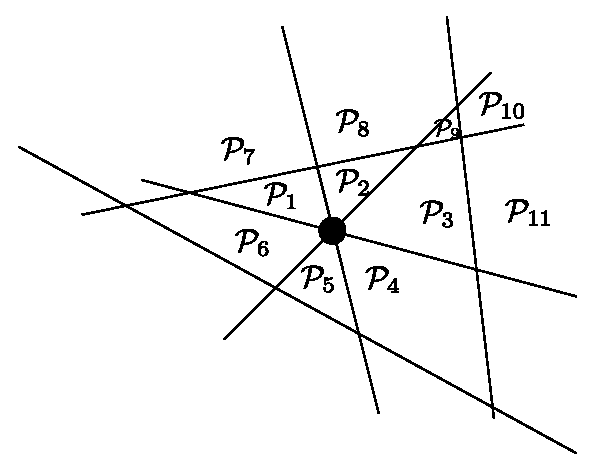
\includegraphics[width=0.4\textwidth]{./global_convergence1.eps}
	\caption{The origin (black dot) has to be the shared vertex of the neighbouring pieces ($\mathcal{P}_1, \mathcal{P}_2, ..., \mathcal{P}_6$ in the figure), it cannot be in the strict interior of any piece.}
	\label{fig:global_convergence1}
\end{figure}
As $V(0)=0$, we know that $h_i = 0$ if $\mathcal{P}_i$ has the origin as a vertex.

Next we show that we can construct a piecewise linear Lyapunov function $\bar{V}$ using the piecewise affine Lyapunov function $V$. The procedure is as follows
\begin{enumerate}
	\item Select each of the piece $\mathcal{P}_i$ that neighbours the origin.
	\item For each of the piece $\mathcal{P}_i$ in step 1, compute the cone of $\mathcal{P}_i = \{x | C_ix\le d_i\}$, by keeping the boundaries of $\mathcal{P}_i$ that contain the origin, and remove the boundaries that don't contain the origin. We denote this conic region as $\bar{\mathcal{P}}_i=\{x|\bar{C}_i\le 0\}$.
	\item Within each of the conic region $\bar{\mathcal{P}}_i$, the new Lyapunov function is defined as $\bar{V}(x) = g_i^Tx \text{ if } \bar{C}_i \le 0$. 
\end{enumerate}
This procedure is shown in Fig.\ref{fig:global_convergence2}.
\begin{figure}
	\centering
	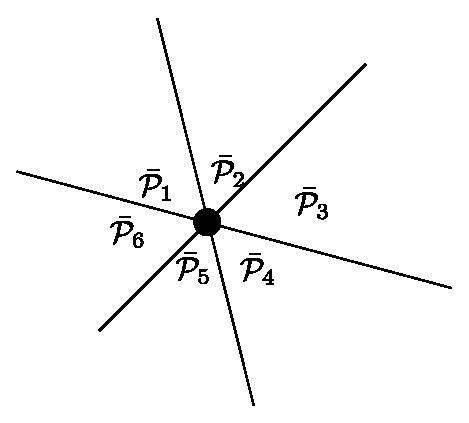
\includegraphics[width=0.4\textwidth]{./global_convergence2.eps}
	\caption{We construct the new Lyapunov function, by first forming the conic region of each piece that neighbours the origin. Hence we extend the region $\mathcal{P}_1, ...\mathcal{P}_6$ to infinity, and remove the pieces that don't neighbour the origin ($\mathcal{P}_7, ...\mathcal{P}_{11}$).}
	\label{fig:global_convergence2}
\end{figure}
Now we need to prove that $\bar{V}$ is a valid Lyapunov function. Notice that in the polyhedron piece $\mathcal{P}_i$, the Lyapunov function $V(x)$ is $V(x) = g_i^Tx$. Now for any state $x$ in $\mathcal{P}_i$, we shoot a ray starting from the origin and passing $x$. We denote the state on this ray as $kx, k > 0$. Obviously this entire ray is in the conic piece $\bar{\mathcal{P}}_i$ (by the definition of the cone). We also know that $\bar{V}(kx) = k\bar{V}(x) = kV(x)>0$. The first equality is because the function $\bar{V}$ is linear inside each piece, the second equality is because $\bar{V}(x) = V(x) \text{ if } x\in\mathcal{P}_i$. Finally, we know that $\dot{\bar{V}}(kx) = k\dot{\bar{V}}(x) = k\dot{V}(x) < 0$. The first equality is because inside each conic piece $\partial V/\partial x$ is a constant, and the dynamics scales proportionally w.r.t $k$ ($f(kx) = kf(x)$).The second equality is because $\bar{V}(x)$ is the same as $V(x)$ in the polyhedron region $\mathcal{P}_i$. As a result, we prove that this new function $\bar{V}(x)$ is a valid Lyapunov function. This piecewise linear function $\bar{V}$ can be represented by neural network without bias term.
\end{document}
